\documentclass[a4paper]{article}
\usepackage{color}              %Farben, f.r \definecolor{}
\usepackage{amssymb}            %Mathematische Symbole
\usepackage{amsthm}             %Besseres \newtheorem
\usepackage{amsmath}           %Mathematische Umgebungen
\usepackage{mathtools}          %\xRightarrow, etc
\usepackage{mathrsfs}           %enthaelt \mathscr
\usepackage{graphicx}
\usepackage{enumerate}          % in-place numerations def.
\usepackage{fullpage}

\usepackage{array}
%\usepackage{multicol}
%\usepackage[notref,notcite]{showkeys}
%\usepackage{algorithm,algorithmic}
\usepackage{color}

\usepackage{graphicx}
\usepackage{xypic}
\entrymodifiers={+!!<0pt,\fontdimen22\textfont2>}
\usepackage[all]{xy}

\usepackage{float}
\usepackage{tikz}
\usepackage{tikz-cd}
\usepackage{tikz,fullpage}
\usetikzlibrary{arrows,%
                petri,%
                topaths}%
\usepackage{tkz-berge}
\usepackage[position=top]{subfig}
\usetikzlibrary{shapes.geometric}
\usetikzlibrary{decorations.markings}

\newtheoremstyle{myremark} % name
    {7pt}                    % Space above
    {7pt}                    % Space below
    {}  	                 % Body font
    {}                           % Indent amount
    {\bf}       	         % Theorem head font
    {.}                          % Punctuation after theorem head
    {.5em}                       % Space after theorem head
    {}  % Theorem head spec (can be left empty, meaning ‘normal’)

\theoremstyle{plain}
\newtheorem{lemma}{Lemma}
\newtheorem{theorem}[lemma]{Theorem}
\newtheorem{fact}[lemma]{Fact}
\newtheorem{definition}[lemma]{Definition}
\newtheorem{corollary}[lemma]{Corollary}
\newtheorem{proposition}[lemma]{Proposition}
\newtheorem{conjecture}[lemma]{Conjecture}
\newtheorem{observation}[lemma]{Observation}
\newtheorem{problem}[lemma]{Problem}
\newtheorem{notation}[lemma]{Notation}
\newtheorem*{claim}{Claim}

\theoremstyle{myremark}
\newtheorem{remark}[lemma]{Remark}
\newtheorem{example}[lemma]{Example}
\newtheorem{exercise}[lemma]{Exercise}
\newtheorem{algorithm}[lemma]{Algorithm}
\newtheorem{application}[lemma]{Application}
\newtheorem*{goal}{Goal}

%%%%%% EDIT HERE: %%%%%%%%%%%
\newcommand{\LECTURENUMBER}{0}
\newcommand{\LECTURETITLE}{Short title}
\newcommand{\LECTURESCRIBE}{Your name}

%% Dokument Beginn %%%%%%%%%%%%%%%%%%%%%%%%%%%%%%%%%%%%%%%%%%%%%%%%%%%%%%%%
\begin{document}
\thispagestyle{empty}

\begin{center}
	{\Large\bf Graph coloring}\\
	{\bf Lecture notes, vol. 10 \\ Hall's marriage theorem and Edge coloring vs. 4-color theorem.}\\
\end{center}
Lecturer: Michal Adamaszek \hfill Student: Hugr\'un Fj\'ola Hafsteinsd\'ottir
\begin{center}
\line(1,0){450}
\end{center}

%%%%%%% EDIT ALSO BELOW: %%%%%%%%%%%%%%%%

In the next pages, $G$ is always a graph, $V(G)$ its set of vertices and $E(G)$ its set of edges. 

%\begin{remark}
%In Homeworkset 1, one can easily solve problem 4 by Brooks theorem.
%\end{remark}

\section*{Hall's marriage theorem}
$G$-bipartite graph with parts $A,B$. Suppose for any $X\subseteq A$, $|N(X)|\geq |X|$ where $N(X)=\bigcup_{x\in X}N_G(x)$. Then $G$ has a matching of size $|A|$.

\emph{"Application":} Split 52 cards into 13 piles of 4 cards each. Then we can choose 1 card from each pile, so that we have one card of each rank: $A,2,3,\dots,K$. Construct a bipartite graph $G$, $V(G)=R\cup P$ ($R$ --- ranks and $P$ --- piles). Edges are $rp\in E(G)$ if pile $p$ has a card of rank $r$. A matching in $G$ with 13 edges determines a bijection $P\longleftrightarrow R$

\begin{center}
    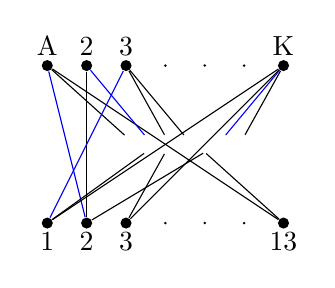
\begin{tikzpicture} 
    \draw  
        node[fill=black,circle,inner sep=0pt,minimum size=4pt] (rA) at (-1,0) {} (-1,0) node [text=black,above] {A}
        node[fill=black,circle,inner sep=0pt,minimum size=4pt] (r2) at (-0.5,0) {} (-0.5,0) node [text=black,above] {2}
        node[fill=black,circle,inner sep=0pt,minimum size=4pt] (r3) at (0,0) {} (0,0) node [text=black,above] {3}
        node[fill=black,circle,inner sep=0pt,minimum size=1pt] (r4) at (0.5,0) {}% (0.5,0) node [text=black,above] {A}
        node[fill=black,circle,inner sep=0pt,minimum size=1pt] (r5) at (1,0) {}% (-0.5,0) node [text=black,above] {2}
        node[fill=black,circle,inner sep=0pt,minimum size=1pt] (r6) at (1.5,0) {}% (0,0) node [text=black,above] {3}
        node[fill=black,circle,inner sep=0pt,minimum size=4pt] (rK) at (2,0) {} (2,0) node [text=black,above] {K}

        node[fill=white,circle,inner sep=0pt,minimum size=1pt] (n1) at (-1,-0.9) {}% (-0.5,0) node [text=black,above] {2}
        node[fill=white,circle,inner sep=0pt,minimum size=1pt] (n2) at (-0.75,-0.9) {}% (-0.5,0) node [text=black,above] {2}
        node[fill=white,circle,inner sep=0pt,minimum size=1pt] (n3) at (-0.5,-0.9) {}% (-0.5,0) node [text=black,above] {2}
        node[fill=white,circle,inner sep=0pt,minimum size=1pt] (n4) at (-0.25,-0.9) {}% (-0.5,0) node [text=black,above] {2}
        node[fill=white,circle,inner sep=0pt,minimum size=1pt] (n5) at (0,-0.9) {}% (0.5,0) node [text=black,above] {A}
        node[fill=white,circle,inner sep=0pt,minimum size=1pt] (n6) at (0.25,-0.9) {}% (-0.5,0) node [text=black,above] {2}
        node[fill=white,circle,inner sep=0pt,minimum size=1pt] (n7) at (0.5,-0.9) {}% (-0.5,0) node [text=black,above] {2}
        node[fill=white,circle,inner sep=0pt,minimum size=1pt] (n8) at (0.75,-0.9) {}% (0.5,0) node [text=black,above] {A}
        node[fill=white,circle,inner sep=0pt,minimum size=1pt] (n9) at (1,-0.9) {}% (0.5,0) node [text=black,above] {A}
        node[fill=white,circle,inner sep=0pt,minimum size=1pt] (n10) at (1.25,-0.9) {}% (0.5,0) node [text=black,above] {A}
        node[fill=white,circle,inner sep=0pt,minimum size=1pt] (n11) at (1.5,-0.9) {}% (0.5,0) node [text=black,above] {A}
        node[fill=white,circle,inner sep=0pt,minimum size=1pt] (n12) at (1.75,-0.9) {}% (0,0) node [text=black,above] {3}
        node[fill=white,circle,inner sep=0pt,minimum size=1pt] (n13) at (2,-0.9) {}% (0,0) node [text=black,above] {3}
        
        node[fill=white,circle,inner sep=0pt,minimum size=1pt] (m1) at (-1,-1.1) {}% (-0.5,0) node [text=black,above] {2}
        node[fill=white,circle,inner sep=0pt,minimum size=1pt] (m2) at (-0.75,-1.1) {}% (-0.5,0) node [text=black,above] {2}
        node[fill=white,circle,inner sep=0pt,minimum size=1pt] (m3) at (-0.5,-1.1) {}% (-0.5,0) node [text=black,above] {2}
        node[fill=white,circle,inner sep=0pt,minimum size=1pt] (m4) at (-0.25,-1.1) {}% (-0.5,0) node [text=black,above] {2}
        node[fill=white,circle,inner sep=0pt,minimum size=1pt] (m5) at (0,-1.1) {}% (0.5,0) node [text=black,above] {A}
        node[fill=white,circle,inner sep=0pt,minimum size=1pt] (m6) at (0.25,-1.1) {}% (-0.5,0) node [text=black,above] {2}
        node[fill=white,circle,inner sep=0pt,minimum size=1pt] (m7) at (0.5,-1.1) {}% (-0.5,0) node [text=black,above] {2}
        node[fill=white,circle,inner sep=0pt,minimum size=1pt] (m8) at (0.75,-1.1) {}% (0.5,0) node [text=black,above] {A}
        node[fill=white,circle,inner sep=0pt,minimum size=1pt] (m9) at (1,-1.1) {}% (0.5,0) node [text=black,above] {A}
        node[fill=white,circle,inner sep=0pt,minimum size=1pt] (m10) at (1.25,-1.1) {}% (0.5,0) node [text=black,above] {A}
        node[fill=white,circle,inner sep=0pt,minimum size=1pt] (m11) at (1.5,-1.1) {}% (0.5,0) node [text=black,above] {A}
        node[fill=white,circle,inner sep=0pt,minimum size=1pt] (m12) at (1.75,-1.1) {}% (0,0) node [text=black,above] {3}
        node[fill=white,circle,inner sep=0pt,minimum size=1pt] (m13) at (2,-1.1) {}% (0,0) node [text=black,above] {3}
        
        node[fill=black,circle,inner sep=0pt,minimum size=4pt] (p1) at (-1,-2) {} (-1,-2) node [text=black,below] {1}
        node[fill=black,circle,inner sep=0pt,minimum size=4pt] (p2) at (-0.5,-2) {} (-0.5,-2) node [text=black,below] {2}
        node[fill=black,circle,inner sep=0pt,minimum size=4pt] (p3) at (0,-2) {} (0,-2) node [text=black,below] {3}
        node[fill=black,circle,inner sep=0pt,minimum size=1pt] (p4) at (0.5,-2) {}% (0.5,0) node [text=black,above] {A}
        node[fill=black,circle,inner sep=0pt,minimum size=1pt] (p5) at (1,-2) {}% (-0.5,0) node [text=black,above] {2}
        node[fill=black,circle,inner sep=0pt,minimum size=1pt] (p6) at (1.5,-2) {}% (0,0) node [text=black,above] {3}
        node[fill=black,circle,inner sep=0pt,minimum size=4pt] (p13) at (2,-2) {} (2,-2) node [text=black,below] {13}
        ;
    
    \draw [color=blue] (rA) -- (p2) node {};
    \draw [color=black] (rA) -- (n5) node {};    
    \draw [color=black] (rA) -- (p13) node {};
    \draw [color=blue] (r2) -- (n6) node {};
    \draw [color=black] (r2) -- (p2) node {};
    \draw [color=blue] (r3) -- (p1) node {};
    \draw [color=black] (r3) -- (n7) node {};
    \draw [color=black] (r3) -- (n8) node {};
    \draw [color=black] (rK) -- (p1) node {};
    \draw [color=black] (rK) -- (p3) node {};
    \draw [color=blue] (rK) -- (n10) node {};
    \draw [color=black] (rK) -- (n11) node {};
    \draw [color=black] (p1) -- (m6) node {};
    \draw [color=black] (p2) -- (m9) node {};
    \draw [color=black] (p3) -- (m7) node {};
    \draw [color=black] (p13) -- (m9) node {};


    \end{tikzpicture}
    \end{center}

How does this connect to Hall's Theorem? Take any subset $X\subseteq R$. $X$ represents $4\cdot|X|$ actual cards. These cards occupy $\geq |X|$ piles. This is exactly the statement $|N(X)|\geq|X|$, so Hall's theorem applies, and we have a matching of size 13. It's convenient now to use a \emph{multigraph}, where many edges are allowed between two vertices


\begin{center}
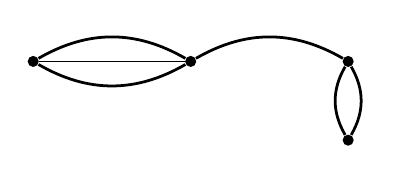
\begin{tikzpicture} 
\draw 
    node[fill,circle,inner sep=0pt,minimum size=4pt] (n1) at (-1,0) {} 
	node[fill,circle,inner sep=0pt,minimum size=4pt] (n2) at (1,0) {}
	node[fill,circle,inner sep=0pt,minimum size=4pt] (n3) at (3,0) {}
	node[fill,circle,inner sep=0pt,minimum size=4pt] (n4) at (3,-1) {}
    ;
\draw
    [line width = 1 pt, black, -, bend right] (n1) edge node {} (n2)
	[line width = 1 pt, black, -, bend left] (n1) edge node {} (n2)
	[line width = 1 pt, black, -, bend left] (n2) edge node {} (n3)
	[line width = 1 pt, black, -, bend right] (n3) edge node {} (n4)
	[line width = 1 pt, black, -, bend left] (n3) edge node {} (n4)
	;
\draw [color=black] (n1) -- (n2) node {};
\end{tikzpicture}
\end{center}



In our example I could take a bipartite multigraph $G$ with one edge for every physical card 

\begin{center}
    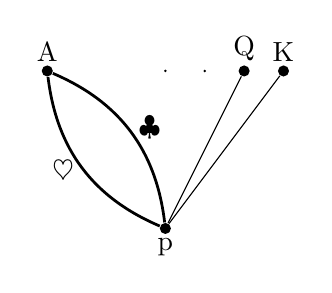
\begin{tikzpicture} 
    \draw  
        node[fill=black,circle,inner sep=0pt,minimum size=4pt] (rA) at (-1,0) {} (-1,0) node [text=black,above] {A}
        node[fill=black,circle,inner sep=0pt,minimum size=1pt] (r4) at (0.5,0) {}% (0.5,0) node [text=black,above] {A}
        node[fill=black,circle,inner sep=0pt,minimum size=1pt] (r5) at (1,0) {}% (-0.5,0) node [text=black,above] {2}
        node[fill=black,circle,inner sep=0pt,minimum size=4pt] (rQ) at (1.5,0) {} (1.5,0) node [text=black,above] {Q}
        node[fill=black,circle,inner sep=0pt,minimum size=4pt] (rK) at (2,0) {} (2,0) node [text=black,above] {K}
        
        node[fill=black,circle,inner sep=0pt,minimum size=4pt] (p) at (0.5,-2) {} (0.5,-2) node [text=black,below] {p}
        ;
    
    \draw
    [line width = 1 pt, black, -, bend right] (rA) edge node {} (p) (0.3,-1) node [above] {$\clubsuit$}
	[line width = 1 pt, black, -, bend left] (rA) edge node {} (p) (-0.8,-1) node [below] {$\heartsuit$}
	;
    
    \draw [color=black] (rQ) -- (p) node {};
    \draw [color=black] (rK) -- (p) node {};    
    
\end{tikzpicture}
\end{center}

In this multigraph every vertex has a degree 4.

\begin{theorem}
If $G$ is a $d$-regular bipartite multigraph, then $\chi'(G)=d$.
\end{theorem}

\begin{proof}
$V(G)=A\cup B$ - parts of the bipartition. $|A|=|B|=n$, because $|E(G)|=d\cdot |A|=d\cdot |B|$.

\emph{Induction on d:}
\begin{itemize}
    \item $d=1:$ $G$ itself is a matching
    \item $d\geq 2:$ Take any $X\subseteq A$ and let $e_X$ be the number of edges in $G[X,N(X)]$

    $d\cdot |X|=e_X\leq d\cdot |N(X)|$, so $|X|\leq |N(X)|$. 
    
    By Hall's Theorem, $G$ has a matching of size $n$, $M\subseteq E(G)$. Since $G-M$ is a $(d-1)$-regular multigraph, by induction $\chi'(G)\leq 1 + (d-1) = d$.
\end{itemize}
\end{proof}

\begin{theorem}(K\"onig)
If $G$ is a bipartite multigraph, then $\chi'(G)=\Delta (G)$.
\end{theorem}

\begin{proof}
$V(G)=A\cup B$. We can assume $|A|=|B|=n$. (If not, then add extra isolated vertices to the smaller part). Write $\Delta := \Delta(G)$. If $A$ has a vertex $v$ of degree $<\Delta$, then also $B$ has some vertex of degree $<\Delta$, call it $u$. (Because existence of $v$ $\Rightarrow |E|<\Delta\cdot n$). Add a new edge $uv$ to the graph. This process ends with $\Delta$-regular bipartite $H$ such that
$$
V(H) = V(G),\,E(G)\subseteq E(H)
$$
By previous theorem, $\chi'(G)\leq \chi'(H)=\Delta$
\end{proof}

\section*{Edge coloring vs. the 4-color theorem.}

Suppose $G$ is a planar triangulation (a planar graph embedded so that all faces are triangles). 

\begin{center}
    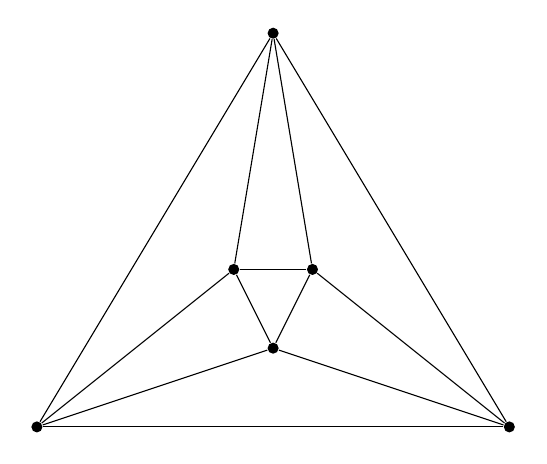
\begin{tikzpicture} 
    \draw  
        node[fill=black,circle,inner sep=0pt,minimum size=4pt] (v1) at (0,2) {} %(0,2) node [text=black,above] {v1}
        node[fill=black,circle,inner sep=0pt,minimum size=4pt] (v2) at (-3,-3) {}% (-3,-3) node [text=black,above] {v2}
        node[fill=black,circle,inner sep=0pt,minimum size=4pt] (v3) at (3,-3) {}% (3,-3) node [text=black,above] {v3}
        node[fill=black,circle,inner sep=0pt,minimum size=4pt] (u1) at (0,-2) {}% (0,-2) node [text=black,above] {u1}
        node[fill=black,circle,inner sep=0pt,minimum size=4pt] (u2) at (-0.5,-1) {}% (-0.5,-1) node [text=black,above] {u2}
        node[fill=black,circle,inner sep=0pt,minimum size=4pt] (u3) at (0.5,-1) {}% (0.5,-1) node [text=black,above] {u3}
        ;

    \draw [color=black] (v1) -- (v2) node {};
    \draw [color=black] (v1) -- (v3) node {};
    \draw [color=black] (v2) -- (v3) node {};
    \draw [color=black] (u1) -- (u2) node {};
    \draw [color=black] (u1) -- (u3) node {};
    \draw [color=black] (u2) -- (u3) node {};
    
    \draw [color=black] (v1) -- (u2) node {};
    \draw [color=black] (v1) -- (u3) node {};
    \draw [color=black] (v2) -- (u2) node {};
    \draw [color=black] (v2) -- (u1) node {};
    \draw [color=black] (v3) -- (u3) node {};
    \draw [color=black] (v3) -- (u1) node {};
    
\end{tikzpicture}
\end{center}

\begin{definition}
The dual graph $G^*$ of $G$ is defined by the conditions: $V(G^*)=$ set of faces of the given embedding of $G$. $F_1F_2\in E(G^*)$ if $F_1,F_2$ share a common edge. (We will usually represent each vertex of $G^*$ as a point inside the corresponding face)

\begin{center}
    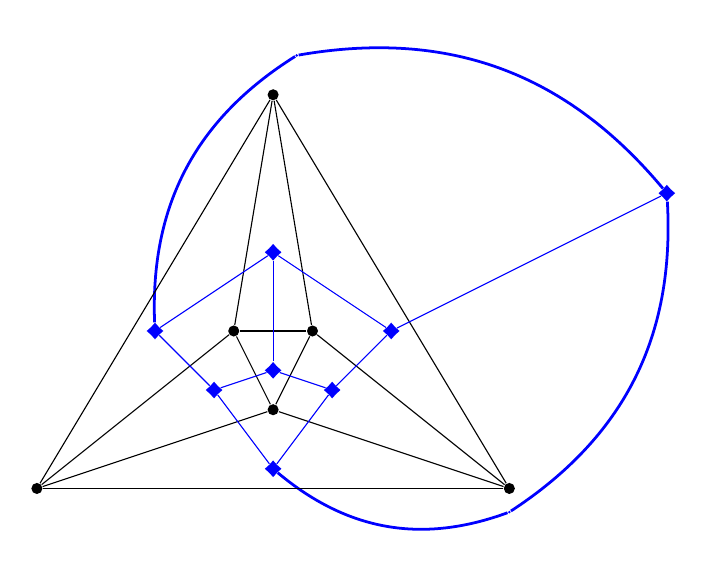
\begin{tikzpicture} 
    \draw  
        node[fill=black,circle,inner sep=0pt,minimum size=4pt] (v1) at (0,2) {} %(0,2) node [text=black,above] {v1}
        node[fill=black,circle,inner sep=0pt,minimum size=4pt] (v2) at (-3,-3) {}% (-3,-3) node [text=black,above] {v2}
        node[fill=black,circle,inner sep=0pt,minimum size=4pt] (v3) at (3,-3) {}% (3,-3) node [text=black,above] {v3}
        node[fill=black,circle,inner sep=0pt,minimum size=4pt] (u1) at (0,-2) {}% (0,-2) node [text=black,above] {u1}
        node[fill=black,circle,inner sep=0pt,minimum size=4pt] (u2) at (-0.5,-1) {}% (-0.5,-1) node [text=black,above] {u2}
        node[fill=black,circle,inner sep=0pt,minimum size=4pt] (u3) at (0.5,-1) {}% (0.5,-1) node [text=black,above] {u3}
        
        node[fill=blue,star,star points=4,inner sep=0pt,minimum size=6pt] (f1) at (0,-1.5) {}% (0,-1.5) node [text=black,above] {f1}
        node[fill=blue,star,star points=4,inner sep=0pt,minimum size=6pt] (f2) at (0,0) {}% (0,0) node [text=black,above] {f2}
        node[fill=blue,star,star points=4,inner sep=0pt,minimum size=6pt] (f3) at (1.5,-1) {}% (1.5,-1) node [text=black,above] {f3}
        node[fill=blue,star,star points=4,inner sep=0pt,minimum size=6pt] (f4) at (-1.5,-1) {}% (-1.5,-1) node [text=black,above] {f4}
        node[fill=blue,star,star points=4,inner sep=0pt,minimum size=6pt] (f5) at (0,-2.75) {}% (0,-2.75) node [text=black,above] {f5}
        node[fill=blue,star,star points=4,inner sep=0pt,minimum size=6pt] (f6) at (0.75,-1.75) {}% (0.75,-1.75) node [text=black,above] {f6}
        node[fill=blue,star,star points=4,inner sep=0pt,minimum size=6pt] (f7) at (-0.75,-1.75) {}% (-0.75,-1.75) node [text=black,above] {f7}
        node[fill=blue,star,star points=4,inner sep=0pt,minimum size=6pt] (f8) at (5,0.75) {}% (5,0.75) node [text=black,above] {f8}
        
        node[fill=blue,circle,inner sep=0pt,minimum size=1pt] (a1) at (0.3,2.5) {}% (0.3,2.5) node [text=black,above] {a1}
        node[fill=blue,circle,inner sep=0pt,minimum size=1pt] (a2) at (3,-3.3) {}% (3,-3.3) node [text=black,above] {a2}
        ;
    \draw
    [line width = 1 pt, blue, -, bend right] (f5) edge node {} (a2)
    [line width = 1 pt, blue, -, bend right] (a2) edge node {} (f8)
	[line width = 1 pt, blue, -, bend left] (f4) edge node {} (a1)
	[line width = 1 pt, blue, -, bend left] (a1) edge node {} (f8)
	;
    \draw [color=black] (v1) -- (v2) node {};
    \draw [color=black] (v1) -- (v3) node {};
    \draw [color=black] (v2) -- (v3) node {};
    \draw [color=black] (u1) -- (u2) node {};
    \draw [color=black] (u1) -- (u3) node {};
    \draw [color=black] (u2) -- (u3) node {};
    
    \draw [color=black] (v1) -- (u2) node {};
    \draw [color=black] (v1) -- (u3) node {};
    \draw [color=black] (v2) -- (u2) node {};
    \draw [color=black] (v2) -- (u1) node {};
    \draw [color=black] (v3) -- (u3) node {};
    \draw [color=black] (v3) -- (u1) node {};
    
    \draw [color=blue] (f3) -- (f8) node {};
    
    \draw [color=blue] (f1) -- (f2) node {};
    \draw [color=blue] (f1) -- (f6) node {};
    \draw [color=blue] (f1) -- (f7) node {};
    \draw [color=blue] (f2) -- (f4) node {};
    \draw [color=blue] (f2) -- (f3) node {};
    \draw [color=blue] (f3) -- (f6) node {};
    \draw [color=blue] (f6) -- (f5) node {};
    \draw [color=blue] (f5) -- (f7) node {};
    \draw [color=blue] (f7) -- (f4) node {};

\end{tikzpicture}
\end{center}

\end{definition}

\begin{observation}
By construction $G^*$ has the following properties
\begin{enumerate}
    \item[a)] $G^*$ is 3-regular. (Because every fave has 3 faces neighboring via a common edge)
    \item[b)] $|E(G^*)|=|E(G)|$
    
            In fact every edge $e$ of $G$ determines an edge $e^*$ of $G^*$. 
            
\begin{center}
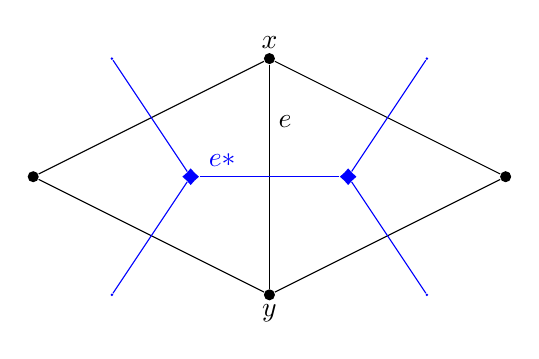
\begin{tikzpicture} 
    \draw  
        node[fill=black,circle,inner sep=0pt,minimum size=4pt] (x) at (0,0) {} (0,0) node [text=black,above] {$x$}
        node[fill=black,circle,inner sep=0pt,minimum size=4pt] (y) at (0,-3) {} (0,-3) node [text=black,below] {$y$}
        node[fill=black,circle,inner sep=0pt,minimum size=4pt] (v1) at (3,-1.5) {} %(0,0) node [text=black,above] {$x$}
        node[fill=black,circle,inner sep=0pt,minimum size=4pt] (v2) at (-3,-1.5) {} %(0,-3) node [text=black,below] {$y$}
        
        node[fill=blue,star,star points=4,inner sep=0pt,minimum size=6pt] (x1) at (1,-1.5) {}% (1.5,-1.5 node [text=black,above] {$x$}
        node[fill=blue,star,star points=4,inner sep=0pt,minimum size=6pt] (y1) at (-1,-1.5) {}% (1.5,-1.5 node [text=black,above] {$x$}
        node[fill=blue,circle,inner sep=0pt,minimum size=1pt] (a1) at (2,0) {}% (0,-3) node [text=black,below] {$y$}
        node[fill=blue,circle,inner sep=0pt,minimum size=1pt] (a2) at (-2,0) {}% (0,-3) node [text=black,below] {$y$}
        node[fill=blue,circle,inner sep=0pt,minimum size=1pt] (a3) at (2,-3) {}% (0,-3) node [text=black,below] {$y$}
        node[fill=blue,circle,inner sep=0pt,minimum size=1pt] (a4) at (-2,-3) {}% (0,-3) node [text=black,below] {$y$}
        ;   
    \draw [color=black] (x) -- (y) node {} (0.2,-1) node [text=black,above] {$e$};
    \draw [color=black] (v1) -- (x) node {};
    \draw [color=black] (v1) -- (y) node {};
    \draw [color=black] (v2) -- (x) node {};
    \draw [color=black] (v2) -- (y) node {};
    
    \draw [color=blue] (x1) -- (y1) node {} (-0.6,-1.5) node [text=blue,above] {$e*$};
    \draw [color=blue] (x1) -- (a1) node {};
    \draw [color=blue] (y1) -- (a2) node {};
    \draw [color=blue] (x1) -- (a3) node {};
    \draw [color=blue] (y1) -- (a4) node {};
    
\end{tikzpicture}
\end{center}
            
    \item[c)] $G^*$ is planar
    \item[d)] Every face of $G^*$ contains exactly one vertex of $G$.

\begin{center}
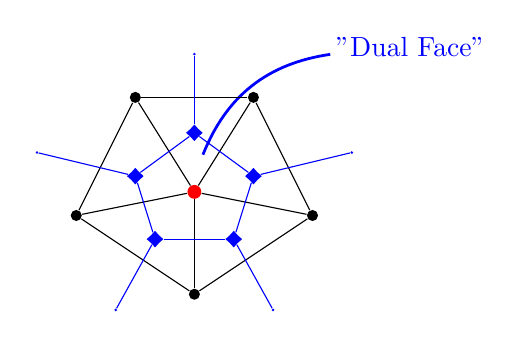
\begin{tikzpicture} 
    \draw  
        node[fill=red,circle,inner sep=0pt,minimum size=5pt] (x) at (0,0) {}% (0,0) node [text=black,above] {$x$}
        node[fill=black,circle,inner sep=0pt,minimum size=4pt] (1) at (0.75,1.2) {}% (0.75,1.2) node [text=black,above] {$1$}
        node[fill=black,circle,inner sep=0pt,minimum size=4pt] (2) at (1.5,-0.3) {}% (1.5,0) node [text=black,above] {$2$}
        node[fill=black,circle,inner sep=0pt,minimum size=4pt] (3) at (0,-1.3) {}% (0,-1.3) node [text=black,above] {$3$}        
        node[fill=black,circle,inner sep=0pt,minimum size=4pt] (4) at (-1.5,-0.3) {}% (-1.5,0) node [text=black,above] {$4$}
        node[fill=black,circle,inner sep=0pt,minimum size=4pt] (5) at (-0.75,1.2) {}% (-0.75,1.2) node [text=black,above] {$5$}
        
        node[fill=blue,star,star points=4,inner sep=0pt,minimum size=6pt] (f1) at (0,0.75) {}% (0,0.75) node [text=black,above] {$1$}
        node[fill=blue,star,star points=4,inner sep=0pt,minimum size=6pt] (f2) at (0.75,0.2) {}% (0.75,0.2) node [text=black,above] {$2$}
        node[fill=blue,star,star points=4,inner sep=0pt,minimum size=6pt] (f3) at (0.5,-0.6) {}% (0.5,-0.6) node [text=black,above] {$3$}
        node[fill=blue,star,star points=4,inner sep=0pt,minimum size=6pt] (f4) at (-0.5,-0.6) {}% (-0.5,-0.6) node [text=black,above] {$4$}
        node[fill=blue,star,star points=4,inner sep=0pt,minimum size=6pt] (f5) at (-0.75,0.2) {}% (-0.75,0.2) node [text=black,above] {$5$}
        
        node[fill=blue,circle,inner sep=0pt,minimum size=1pt] (a1) at (0,1.75) {}% (0,1.6) node [text=black,above] {$1$}
        node[fill=blue,circle,inner sep=0pt,minimum size=1pt] (a2) at (2,0.5) {}% (2,0.5) node [text=black,above] {$2$}
        node[fill=blue,circle,inner sep=0pt,minimum size=1pt] (a3) at (1,-1.5) {}% (1,-1.5) node [text=black,above] {$3$}
        node[fill=blue,circle,inner sep=0pt,minimum size=1pt] (a4) at (-1,-1.5) {}% (-1,-1.5) node [text=black,above] {$4$}
        node[fill=blue,circle,inner sep=0pt,minimum size=1pt] (a5) at (-2,0.5) {}% (-2,0.5) node [text=black,above] {$5$}
        
        node[fill=white,circle,inner sep=0pt,minimum size=1pt] (l1) at (1.75,1.75) {} (2.75,1.6) node [text=blue,above] {\text{"Dual Face"}}
        node[fill=white,circle,inner sep=0pt,minimum size=1pt] (l2) at (0.1,0.45) {}% (0,0) node [text=black,above] {$x$}
        ;   
    \draw [line width = 1 pt, blue, -, bend left] (l2) edge node {} (l1);

    \draw [color=black] (x) -- (1) node {};
    \draw [color=black] (x) -- (2) node {};
    \draw [color=black] (x) -- (3) node {};
    \draw [color=black] (x) -- (4) node {};
    \draw [color=black] (x) -- (5) node {};
    \draw [color=black] (5) -- (1) node {};
    \draw [color=black] (1) -- (2) node {};
    \draw [color=black] (2) -- (3) node {};
    \draw [color=black] (3) -- (4) node {};
    \draw [color=black] (4) -- (5) node {};

    \draw [color=blue] (f1) -- (f2) node {};
    \draw [color=blue] (f2) -- (f3) node {};
    \draw [color=blue] (f3) -- (f4) node {};
    \draw [color=blue] (f4) -- (f5) node {};
    \draw [color=blue] (f5) -- (f1) node {};
    
    \draw [color=blue] (f1) -- (a1) node {};
    \draw [color=blue] (f2) -- (a2) node {};
    \draw [color=blue] (f3) -- (a3) node {};
    \draw [color=blue] (f4) -- (a4) node {};
    \draw [color=blue] (f5) -- (a5) node {};
    
\end{tikzpicture}
\end{center}

    \item[e)]   $|V(G^*)|=|F(G)|,\ |E(G^*)|=|E(G)|,\ |F(G^*)|=|V(G)|.$
\end{enumerate}
\end{observation}

\begin{theorem}
\emph{(Tait '1878, Tait's attempt at the four-color problem).}

Suppose $G$ is a planar triangulation. TFAE:
\begin{enumerate}
    \item[a)] $G$ is 4-colorable
    \item[b)] $G^*$ is 3-colorable
\end{enumerate}
\end{theorem}

\begin{proof}
\begin{itemize}
    \item \emph{a) $\Rightarrow$ b)}
    
    Take a 4-coloring $c:V(G)\rightarrow \{00,01,10,11\}$. If $e\in E(G)$, $e=xy$ then we color $e^*$ with color $f(e^*)=c(x)\oplus c(y)$.

\begin{center}
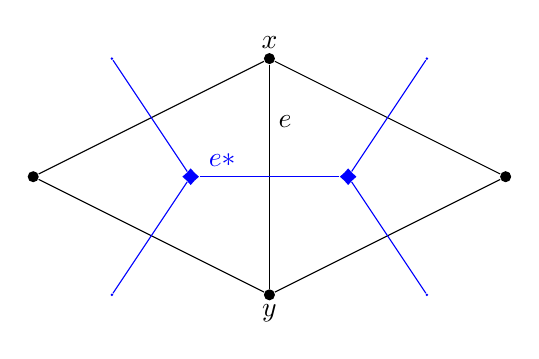
\begin{tikzpicture} 
    \draw  
        node[fill=black,circle,inner sep=0pt,minimum size=4pt] (x) at (0,0) {} (0,0) node [text=black,above] {$x$}
        node[fill=black,circle,inner sep=0pt,minimum size=4pt] (y) at (0,-3) {} (0,-3) node [text=black,below] {$y$}
        node[fill=black,circle,inner sep=0pt,minimum size=4pt] (v1) at (3,-1.5) {} %(0,0) node [text=black,above] {$x$}
        node[fill=black,circle,inner sep=0pt,minimum size=4pt] (v2) at (-3,-1.5) {} %(0,-3) node [text=black,below] {$y$}
        
        node[fill=blue,star,star points=4,inner sep=0pt,minimum size=6pt] (x1) at (1,-1.5) {}% (1.5,-1.5 node [text=black,above] {$x$}
        node[fill=blue,star,star points=4,inner sep=0pt,minimum size=6pt] (y1) at (-1,-1.5) {}% (1.5,-1.5 node [text=black,above] {$x$}
        node[fill=blue,circle,inner sep=0pt,minimum size=1pt] (a1) at (2,0) {}% (0,-3) node [text=black,below] {$y$}
        node[fill=blue,circle,inner sep=0pt,minimum size=1pt] (a2) at (-2,0) {}% (0,-3) node [text=black,below] {$y$}
        node[fill=blue,circle,inner sep=0pt,minimum size=1pt] (a3) at (2,-3) {}% (0,-3) node [text=black,below] {$y$}
        node[fill=blue,circle,inner sep=0pt,minimum size=1pt] (a4) at (-2,-3) {}% (0,-3) node [text=black,below] {$y$}
        ;   
    \draw [color=black] (x) -- (y) node {} (0.2,-1) node [text=black,above] {$e$};
    \draw [color=black] (v1) -- (x) node {};
    \draw [color=black] (v1) -- (y) node {};
    \draw [color=black] (v2) -- (x) node {};
    \draw [color=black] (v2) -- (y) node {};
    
    \draw [color=blue] (x1) -- (y1) node {} (-0.6,-1.5) node [text=blue,above] {$e*$};
    \draw [color=blue] (x1) -- (a1) node {};
    \draw [color=blue] (y1) -- (a2) node {};
    \draw [color=blue] (x1) -- (a3) node {};
    \draw [color=blue] (y1) -- (a4) node {};
    
\end{tikzpicture}
\end{center}

    $\oplus$ is the coordinate-wise addition mod 2. (XOR = exclusive or)
    
\begin{align*}
     0\oplus 0 &= 0 = 1\oplus 1 & 01 \oplus 11 &= 10 & & \\
     1\oplus 0 &= 1 = 0\oplus 1 & A\oplus B &= 00 & \text{ iff } A=B
\end{align*}
    
    
    Let's check that $f$ is an edge 3-coloring.
    \begin{itemize}
        \item $f(e^*)\neq 00$ because $c(x)\neq c(y)$, therefore $im(f)	\subseteq\{01,10,11\}$
        \item Take $e^*,f^*\in E(G^*)$ sharing a common vertex

\begin{center}
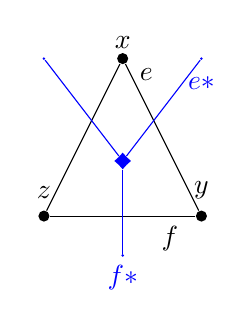
\begin{tikzpicture} 
    \draw  
        node[fill=black,circle,inner sep=0pt,minimum size=4pt] (1) at (0,0) {} (0,0)node [text=black,above] {$x$}
        node[fill=black,circle,inner sep=0pt,minimum size=4pt] (2) at (1,-2) {} (1,-1.9) node [text=black,above] {$y$}
        node[fill=black,circle,inner sep=0pt,minimum size=4pt] (3) at (-1,-2) {} (-1,-1.9) node [text=black,above] {$z$}
        
        node[fill=blue,star,star points=4,inner sep=0pt,minimum size=6pt] (x) at (0,-1.3) {}% (0,-1.3) node [text=black,above] {$x$}
        
        node[fill=blue,circle,inner sep=0pt,minimum size=1pt] (f1) at (1,0) {}% (1,0) node [text=black,above] {$1$}
        node[fill=blue,circle,inner sep=0pt,minimum size=1pt] (f2) at (-1,0) {}% (-1,0) node [text=black,above] {$2$}
        node[fill=blue,circle,inner sep=0pt,minimum size=1pt] (f3) at (0,-2.5) {}% (0,-2.5) node [text=black,above] {$3$}
        ; 

    \draw [color=black] (1) -- (2) node {} (0.3,-0.4) node [text=black,above] {$e$};
    \draw [color=black] (2) -- (3) node {} (0.6,-2) node [text=black,below] {$f$};
    \draw [color=black] (3) -- (1) node {};
    
    \draw [color=blue] (x) -- (f1) node {} (1,-0.1) node [text=blue,below] {$e*$};
    \draw [color=blue] (x) -- (f2) node {} (0,-2.5) node [text=blue,below] {$f*$};
    \draw [color=blue] (x) -- (f3) node {};
\end{tikzpicture}
\end{center}

        $f(e^*)=c(x)\oplus c(y)\neq c(y)\oplus c(z)=f(f^*)$, because $c(x)\neq c(z)$
    \end{itemize}
    
    \item \emph{b) $\Rightarrow$ a)}
    
    Start with a 3-coloring of $E(G^*)$:
    $$
    f:E(G^*)\rightarrow \{1,2,3\}
    $$
    Since $G^*$ is 3-regular, every color appears at every vertex of $G^*$. For $i=1,2$ let $H_i \subseteq G^*$ be the subgraph on the edges $f^{-1}(i)\cup f^{-1}(3)$.
  
\begin{center}
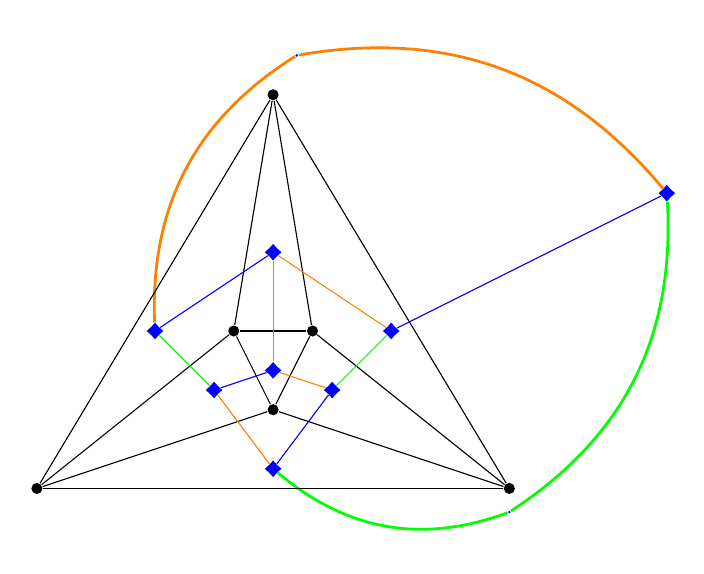
\begin{tikzpicture} 
    \draw  
        node[fill=black,circle,inner sep=0pt,minimum size=4pt] (v1) at (0,2) {} %(0,2) node [text=black,above] {v1}
        node[fill=black,circle,inner sep=0pt,minimum size=4pt] (v2) at (-3,-3) {}% (-3,-3) node [text=black,above] {v2}
        node[fill=black,circle,inner sep=0pt,minimum size=4pt] (v3) at (3,-3) {}% (3,-3) node [text=black,above] {v3}
        node[fill=black,circle,inner sep=0pt,minimum size=4pt] (u1) at (0,-2) {}% (0,-2) node [text=black,above] {u1}
        node[fill=black,circle,inner sep=0pt,minimum size=4pt] (u2) at (-0.5,-1) {}% (-0.5,-1) node [text=black,above] {u2}
        node[fill=black,circle,inner sep=0pt,minimum size=4pt] (u3) at (0.5,-1) {} %(0.6,-1) node [text=black,above] {$v$}
        
        node[fill=blue,star,star points=4,inner sep=0pt,minimum size=6pt] (f1) at (0,-1.5) {}% (0,-1.5) node [text=black,above] {f1}
        node[fill=blue,star,star points=4,inner sep=0pt,minimum size=6pt] (f2) at (0,0) {}% (0,0) node [text=black,above] {f2}
        node[fill=blue,star,star points=4,inner sep=0pt,minimum size=6pt] (f3) at (1.5,-1) {}% (1.5,-1) node [text=black,above] {f3}
        node[fill=blue,star,star points=4,inner sep=0pt,minimum size=6pt] (f4) at (-1.5,-1) {}% (-1.5,-1) node [text=black,above] {f4}
        node[fill=blue,star,star points=4,inner sep=0pt,minimum size=6pt] (f5) at (0,-2.75) {}% (0,-2.75) node [text=black,above] {f5}
        node[fill=blue,star,star points=4,inner sep=0pt,minimum size=6pt] (f6) at (0.75,-1.75) {}% (0.75,-1.75) node [text=black,above] {f6}
        node[fill=blue,star,star points=4,inner sep=0pt,minimum size=6pt] (f7) at (-0.75,-1.75) {}% (-0.75,-1.75) node [text=black,above] {f7}
        node[fill=blue,star,star points=4,inner sep=0pt,minimum size=6pt] (f8) at (5,0.75) {}% (5,0.75) node [text=black,above] {f8}
        
        node[fill=blue,circle,inner sep=0pt,minimum size=1pt] (a1) at (0.3,2.5) {}% (0.3,2.5) node [text=black,above] {a1}
        node[fill=blue,circle,inner sep=0pt,minimum size=1pt] (a2) at (3,-3.3) {}% (3,-3.3) node [text=black,above] {a2}
        ;
    \draw
    [line width = 1 pt, green, -, bend right] (f5) edge node {} (a2)
    [line width = 1 pt, green, -, bend right] (a2) edge node {} (f8)
    ;
	\draw
	[line width = 1 pt, orange, -, bend left] (f4) edge node {} (a1)
	[line width = 1 pt, orange, -, bend left] (a1) edge node {} (f8)
	;
    \draw [color=black] (v1) -- (v2) node {};
    \draw [color=black] (v1) -- (v3) node {};
    \draw [color=black] (v2) -- (v3) node {};
    \draw [color=black] (u1) -- (u2) node {};
    \draw [color=black] (u1) -- (u3) node {};
    \draw [color=black] (u2) -- (u3) node {};
    
    \draw [color=black] (v1) -- (u2) node {};
    \draw [color=black] (v1) -- (u3) node {};
    \draw [color=black] (v2) -- (u2) node {};
    \draw [color=black] (v2) -- (u1) node {};
    \draw [color=black] (v3) -- (u3) node {};
    \draw [color=black] (v3) -- (u1) node {};
    
    \draw [color=blue] (f3) -- (f8) node {};
    
    \draw [color=green] (f1) -- (f2) node {};
    \draw [color=orange] (f1) -- (f6) node {};
    \draw [color=blue] (f1) -- (f7) node {};
    \draw [color=blue] (f2) -- (f4) node {};
    \draw [color=orange] (f2) -- (f3) node {};
    \draw [color=green] (f3) -- (f6) node {};
    \draw [color=blue] (f6) -- (f5) node {};
    \draw [color=orange] (f5) -- (f7) node {};
    \draw [color=green] (f7) -- (f4) node {};

\end{tikzpicture}
\end{center}

    $H_i$ is 2-regular, hence it is a union of cycles.
    Construct a coloring $c:V(G)\rightarrow \{00,01,10,11\}$ as follows:

    \begin{align*}
        c(v) & =x_1x_2 &  \\
         i & =1,2 & x_i=\text{(\# cycles in $H_i$ which contain $v$ inside) }\mod 2 
    \end{align*}
    
    \begin{center}
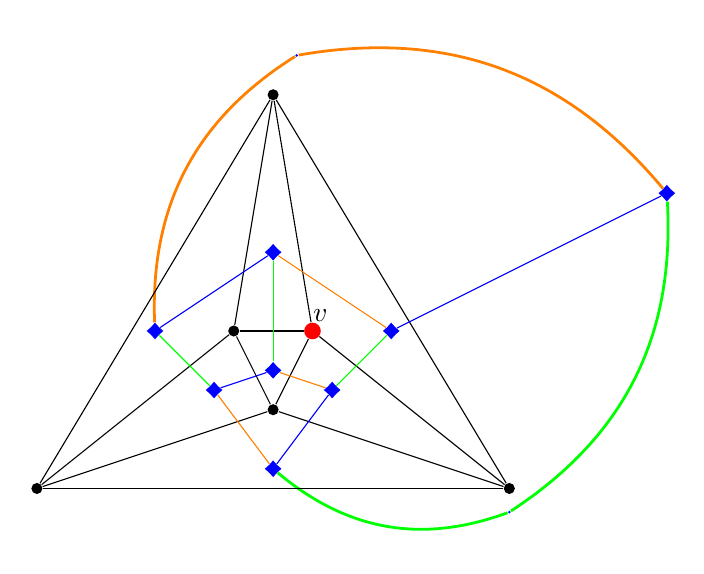
\begin{tikzpicture} 
    \draw  
        node[fill=black,circle,inner sep=0pt,minimum size=4pt] (v1) at (0,2) {} %(0,2) node [text=black,above] {v1}
        node[fill=black,circle,inner sep=0pt,minimum size=4pt] (v2) at (-3,-3) {}% (-3,-3) node [text=black,above] {v2}
        node[fill=black,circle,inner sep=0pt,minimum size=4pt] (v3) at (3,-3) {}% (3,-3) node [text=black,above] {v3}
        node[fill=black,circle,inner sep=0pt,minimum size=4pt] (u1) at (0,-2) {}% (0,-2) node [text=black,above] {u1}
        node[fill=black,circle,inner sep=0pt,minimum size=4pt] (u2) at (-0.5,-1) {}% (-0.5,-1) node [text=black,above] {u2}
        node[fill=red,circle,inner sep=0pt,minimum size=6pt] (u3) at (0.5,-1) {} (0.6,-1) node [text=black,above] {$v$}
        
        node[fill=blue,star,star points=4,inner sep=0pt,minimum size=6pt] (f1) at (0,-1.5) {}% (0,-1.5) node [text=black,above] {f1}
        node[fill=blue,star,star points=4,inner sep=0pt,minimum size=6pt] (f2) at (0,0) {}% (0,0) node [text=black,above] {f2}
        node[fill=blue,star,star points=4,inner sep=0pt,minimum size=6pt] (f3) at (1.5,-1) {}% (1.5,-1) node [text=black,above] {f3}
        node[fill=blue,star,star points=4,inner sep=0pt,minimum size=6pt] (f4) at (-1.5,-1) {}% (-1.5,-1) node [text=black,above] {f4}
        node[fill=blue,star,star points=4,inner sep=0pt,minimum size=6pt] (f5) at (0,-2.75) {}% (0,-2.75) node [text=black,above] {f5}
        node[fill=blue,star,star points=4,inner sep=0pt,minimum size=6pt] (f6) at (0.75,-1.75) {}% (0.75,-1.75) node [text=black,above] {f6}
        node[fill=blue,star,star points=4,inner sep=0pt,minimum size=6pt] (f7) at (-0.75,-1.75) {}% (-0.75,-1.75) node [text=black,above] {f7}
        node[fill=blue,star,star points=4,inner sep=0pt,minimum size=6pt] (f8) at (5,0.75) {}% (5,0.75) node [text=black,above] {f8}
        
        node[fill=blue,circle,inner sep=0pt,minimum size=1pt] (a1) at (0.3,2.5) {}% (0.3,2.5) node [text=black,above] {a1}
        node[fill=blue,circle,inner sep=0pt,minimum size=1pt] (a2) at (3,-3.3) {}% (3,-3.3) node [text=black,above] {a2}
        ;
    \draw
    [line width = 1 pt, green, -, bend right] (f5) edge node {} (a2)
    [line width = 1 pt, green, -, bend right] (a2) edge node {} (f8)
    ;
	\draw
	[line width = 1 pt, orange, -, bend left] (f4) edge node {} (a1)
	[line width = 1 pt, orange, -, bend left] (a1) edge node {} (f8)
	;
    \draw [color=black] (v1) -- (v2) node {};
    \draw [color=black] (v1) -- (v3) node {};
    \draw [color=black] (v2) -- (v3) node {};
    \draw [color=black] (u1) -- (u2) node {};
    \draw [color=black] (u1) -- (u3) node {};
    \draw [color=black] (u2) -- (u3) node {};
    
    \draw [color=black] (v1) -- (u2) node {};
    \draw [color=black] (v1) -- (u3) node {};
    \draw [color=black] (v2) -- (u2) node {};
    \draw [color=black] (v2) -- (u1) node {};
    \draw [color=black] (v3) -- (u3) node {};
    \draw [color=black] (v3) -- (u1) node {};
    
    \draw [color=blue] (f3) -- (f8) node {};
    
    \draw [color=green] (f1) -- (f2) node {};
    \draw [color=orange] (f1) -- (f6) node {};
    \draw [color=blue] (f1) -- (f7) node {};
    \draw [color=blue] (f2) -- (f4) node {};
    \draw [color=orange] (f2) -- (f3) node {};
    \draw [color=green] (f3) -- (f6) node {};
    \draw [color=blue] (f6) -- (f5) node {};
    \draw [color=orange] (f5) -- (f7) node {};
    \draw [color=green] (f7) -- (f4) node {};

\end{tikzpicture}
\end{center}

    \begin{align*}
            H_1 &= f^{-1}(1)\cup f^{-1}(3)\text{, }\,c(v)=(2 \mod 2)(1\mod 2) \\
            H_2 &= f^{-1}(2)\cup f^{-1}(3)   
    \end{align*}
    
The two cycles of $H_1$ that contain $v$ inside are shown below, assuming color 1 is orange and color 3 is green:
\begin{center}
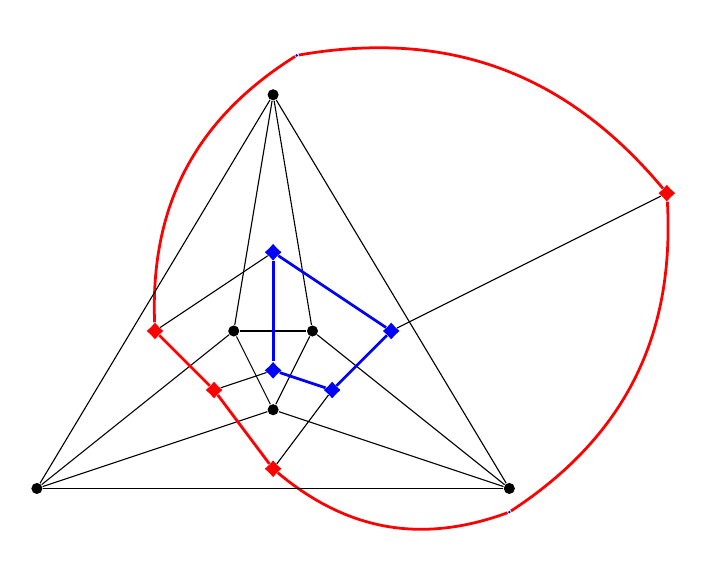
\begin{tikzpicture} 
    \draw  
        node[fill=black,circle,inner sep=0pt,minimum size=4pt] (v1) at (0,2) {} %(0,2) node [text=black,above] {v1}
        node[fill=black,circle,inner sep=0pt,minimum size=4pt] (v2) at (-3,-3) {}% (-3,-3) node [text=black,above] {v2}
        node[fill=black,circle,inner sep=0pt,minimum size=4pt] (v3) at (3,-3) {}% (3,-3) node [text=black,above] {v3}
        node[fill=black,circle,inner sep=0pt,minimum size=4pt] (u1) at (0,-2) {}% (0,-2) node [text=black,above] {u1}
        node[fill=black,circle,inner sep=0pt,minimum size=4pt] (u2) at (-0.5,-1) {}% (-0.5,-1) node [text=black,above] {u2}
        node[fill=black,circle,inner sep=0pt,minimum size=4pt] (u3) at (0.5,-1) {}% (0.6,-1) node [text=black,above] {$v$}
        
        node[fill=blue,star,star points=4,inner sep=0pt,minimum size=6pt] (f1) at (0,-1.5) {}% (0,-1.5) node [text=black,above] {f1}
        node[fill=blue,star,star points=4,inner sep=0pt,minimum size=6pt] (f2) at (0,0) {}% (0,0) node [text=black,above] {f2}
        node[fill=blue,star,star points=4,inner sep=0pt,minimum size=6pt] (f3) at (1.5,-1) {}% (1.5,-1) node [text=black,above] {f3}
        node[fill=red,star,star points=4,inner sep=0pt,minimum size=6pt] (f4) at (-1.5,-1) {}% (-1.5,-1) node [text=black,above] {f4}
        node[fill=red,star,star points=4,inner sep=0pt,minimum size=6pt] (f5) at (0,-2.75) {}% (0,-2.75) node [text=black,above] {f5}
        node[fill=blue,star,star points=4,inner sep=0pt,minimum size=6pt] (f6) at (0.75,-1.75) {}% (0.75,-1.75) node [text=black,above] {f6}
        node[fill=red,star,star points=4,inner sep=0pt,minimum size=6pt] (f7) at (-0.75,-1.75) {}% (-0.75,-1.75) node [text=black,above] {f7}
        node[fill=red,star,star points=4,inner sep=0pt,minimum size=6pt] (f8) at (5,0.75) {}% (5,0.75) node [text=black,above] {f8}
        
        node[fill=blue,circle,inner sep=0pt,minimum size=1pt] (a1) at (0.3,2.5) {}% (0.3,2.5) node [text=black,above] {a1}
        node[fill=blue,circle,inner sep=0pt,minimum size=1pt] (a2) at (3,-3.3) {}% (3,-3.3) node [text=black,above] {a2}
        ;
    \draw
    [line width = 1 pt, red, -, bend right] (f5) edge node {} (a2)
    [line width = 1 pt, red, -, bend right] (a2) edge node {} (f8)
	[line width = 1 pt, red, -, bend left] (f4) edge node {} (a1)
	[line width = 1 pt, red, -, bend left] (a1) edge node {} (f8)
	;
    \draw [color=black] (v1) -- (v2) node {};
    \draw [color=black] (v1) -- (v3) node {};
    \draw [color=black] (v2) -- (v3) node {};
    \draw [color=black] (u1) -- (u2) node {};
    \draw [color=black] (u1) -- (u3) node {};
    \draw [color=black] (u2) -- (u3) node {};
    
    \draw [color=black] (v1) -- (u2) node {};
    \draw [color=black] (v1) -- (u3) node {};
    \draw [color=black] (v2) -- (u2) node {};
    \draw [color=black] (v2) -- (u1) node {};
    \draw [color=black] (v3) -- (u3) node {};
    \draw [color=black] (v3) -- (u1) node {};
    
    \draw [color=black] (f3) -- (f8) node {};
    
    \draw [line width = 1 pt, color=blue] (f1) -- (f2) node {};
    \draw [line width = 1 pt, color=blue] (f1) -- (f6) node {};
    \draw [color=black] (f1) -- (f7) node {};
    \draw [color=black] (f2) -- (f4) node {};
    \draw [line width = 1 pt, color=blue] (f2) -- (f3) node {};
    \draw [line width = 1 pt, color=blue] (f3) -- (f6) node {};
    \draw [color=black] (f6) -- (f5) node {};
    \draw [line width = 1 pt, color=red] (f5) -- (f7) node {};
    \draw [line width = 1 pt, color=red] (f7) -- (f4) node {};

\end{tikzpicture}
\end{center}
    
    \emph{Remember:} A cycle in $H_i$ is a simple polygon in $\mathbb{R}^2$:
    
            \begin{center}
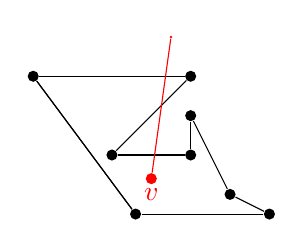
\begin{tikzpicture} 
    \draw  
        node[fill=red,circle,inner sep=0pt,minimum size=1pt] (a) at (1.75,0.5) {} %(0,2) node [text=black,above] {v1}
        
        node[fill=black,circle,inner sep=0pt,minimum size=4pt] (1) at (0,0) {} %(0,2) node [text=black,above] {v1}
        node[fill=black,circle,inner sep=0pt,minimum size=4pt] (2) at (2,0) {} %(0,2) node [text=black,above] {v1}
        node[fill=black,circle,inner sep=0pt,minimum size=4pt] (3) at (1,-1) {} %(0,2) node [text=black,above] {v1}
        node[fill=black,circle,inner sep=0pt,minimum size=4pt] (4) at (1.3,-1.75) {} %(0,2) node [text=black,above] {v1}
        node[fill=black,circle,inner sep=0pt,minimum size=4pt] (5) at (2,-1) {} %(0,2) node [text=black,above] {v1}
        node[fill=black,circle,inner sep=0pt,minimum size=4pt] (6) at (3,-1.75) {} %(0,2) node [text=black,above] {v1}
        node[fill=black,circle,inner sep=0pt,minimum size=4pt] (7) at (2.5,-1.5) {} %(0,2) node [text=black,above] {v1}
        node[fill=black,circle,inner sep=0pt,minimum size=4pt] (8) at (2,-0.5) {} %(0,2) node [text=black,above] {v1}
        node[fill=red,circle,inner sep=0pt,minimum size=4pt] (x) at (1.5,-1.3) {} (1.5,-1.3) node [text=red,below] {$v$}
        ;
    \draw [color=black] (1) -- (2) node {};
    \draw [color=black] (2) -- (3) node {};
    \draw [color=black] (1) -- (4) node {};
    \draw [color=black] (1) -- (4) node {};
    \draw [color=black] (3) -- (5) node {};
    \draw [color=black] (4) -- (6) node {};
    \draw [color=black] (6) -- (7) node {};
    \draw [color=black] (7) -- (8) node {};
    \draw [color=black] (8) -- (5) node {};
    \draw [color=red] (x) -- (a) node {};

\end{tikzpicture}
\end{center}
    
    $v$ is inside the polygon if a generic ray from $v$ intersects the polygon an odd number of times.
    
    This ends the example. Now we will prove that $c$ is a vertex-coloring of $G$. Take $e=uv\in E(G)$. We want to show $c(u)\neq c(v)$. W.l.o.g. suppose that $f(e^*)=1$
    
\begin{center}
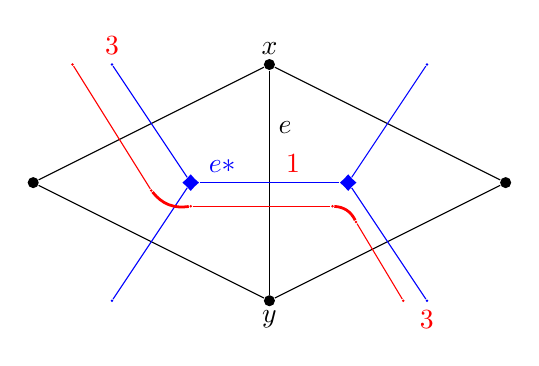
\begin{tikzpicture} 
    \draw  
        node[fill=black,circle,inner sep=0pt,minimum size=4pt] (x) at (0,0) {} (0,0) node [text=black,above] {$x$}
        node[fill=black,circle,inner sep=0pt,minimum size=4pt] (y) at (0,-3) {} (0,-3) node [text=black,below] {$y$}
        node[fill=black,circle,inner sep=0pt,minimum size=4pt] (v1) at (3,-1.5) {} %(0,0) node [text=black,above] {$x$}
        node[fill=black,circle,inner sep=0pt,minimum size=4pt] (v2) at (-3,-1.5) {} %(0,-3) node [text=black,below] {$y$}
        
        node[fill=blue,star,star points=4,inner sep=0pt,minimum size=6pt] (x1) at (1,-1.5) {}% (1.5,-1.5 node [text=black,above] {$x$}
        node[fill=blue,star,star points=4,inner sep=0pt,minimum size=6pt] (y1) at (-1,-1.5) {}% (1.5,-1.5 node [text=black,above] {$x$}
        node[fill=blue,circle,inner sep=0pt,minimum size=1pt] (a1) at (2,0) {}% (0,-3) node [text=black,below] {$y$}
        node[fill=blue,circle,inner sep=0pt,minimum size=1pt] (a2) at (-2,0) {}% (0,-3) node [text=black,below] {$y$}
        node[fill=blue,circle,inner sep=0pt,minimum size=1pt] (a3) at (2,-3) {}% (0,-3) node [text=black,below] {$y$}
        node[fill=blue,circle,inner sep=0pt,minimum size=1pt] (a4) at (-2,-3) {}% (0,-3) node [text=black,below] {$y$}
       
        node[fill=red,circle,inner sep=0pt,minimum size=1pt] (b0) at (-2.5,0) {}% (-2.2,0) node [text=black,below] {$0$} 
        node[fill=red,circle,inner sep=0pt,minimum size=1pt] (b1) at (-1.5,-1.6) {}% (-1.5,-1.6) node [text=black,below] {$1$}
        node[fill=red,circle,inner sep=0pt,minimum size=1pt] (b2) at (-1,-1.8) {}% (-1,-1.8) node [text=black,below] {$2$}
        node[fill=red,circle,inner sep=0pt,minimum size=1pt] (b3) at (0.8,-1.8) {}% (0.8,-1.8) node [text=black,below] {$3$}
        node[fill=red,circle,inner sep=0pt,minimum size=1pt] (b4) at (1.1,-2) {}% (1.1,-2) node [text=black,below] {$4$}
        node[fill=red,circle,inner sep=0pt,minimum size=1pt] (b5) at (1.7,-3) {}% (1.7,-3) node [text=black,below] {$5$}
        
        ;   
        
    \draw [color=black] (x) -- (y) node {} (0.2,-1) node [text=black,above] {$e$};
    \draw [color=black] (v1) -- (x) node {};
    \draw [color=black] (v1) -- (y) node {};
    \draw [color=black] (v2) -- (x) node {};
    \draw [color=black] (v2) -- (y) node {};
    
    \draw [color=blue] (x1) -- (y1) node {} (-0.6,-1.5) node [text=blue,above] {$e*$} (0.3,-1.5) node [text=red,above] {$1$};
    \draw [color=blue] (x1) -- (a1) node {} (-2,0) node [text=red,above] {$3$};
    \draw [color=blue] (y1) -- (a2) node {} (2,-3) node [text=red,below] {$3$};
    \draw [color=blue] (x1) -- (a3) node {};
    \draw [color=blue] (y1) -- (a4) node {};
    
    \draw [color=red] (b0) -- (b1) node {};
    \draw [line width = 1 pt, red, -, bend right] (b1) edge node {} (b2);
    \draw [color=red] (b2) -- (b3) node {};
    \draw [line width = 1 pt, red, -, bend left] (b3) edge node {} (b4);
    \draw [color=red] (b4) -- (b5) node {};
    
\end{tikzpicture}
\end{center}
We know that $e^*$ belongs to some cycle $C$ of $H_1$
    \begin{itemize}
        \item $v$ is inside $C$ and $u$ is outside $C$ or vice versa.
        \item For any other cycle of $H_1$, both $u,v$ are inside or both $u,v$ are outside.
    \end{itemize}
    We can check both caims by counting (mod $2$) the number of times a generic ray from $u$, $v$ intersects a cycle of $H_1$.
    
    By the claim $c(v)$ and $c(u)$ differ in $x_1$. Similarly:
    \begin{enumerate}
        \item[]If $f(e^*)= 2 \rightarrow c(v)$ and $c(u)$ differ in $x_2$
        \item[]If $f(e^*)= 3 \rightarrow c(v)$ and $c(u)$ differ in $x_1$ and $x_2$
    \end{enumerate}
    In any case $c(u)\neq c(v)$, so $c$ is a 4-coloring
\end{itemize}
\end{proof}

\end{document}




